\newpage
\section{Product Requirements}

\subsection{Hardware}
The custom built hardware contains all necessary components integrated on a single \acrfull{pcb}. The hardware needs to comply with the following requirements: 
\begin{itemize}
		\item The hardware shall be based around an \gls{esp32} \acrfull{soc}.
		\item The hardware shall use \acrshort{lan}/\acrshort{wlan} to communicate with the network router.
		\subitem The Ethernet interface shall be galvanically isolated from the rest of the hardware.
		\item The hardware shall have a \acrshort{can} interface to receive \acrshort{fms}-packages from the vehicle.
		\subitem The \acrshort{can} interface shall be galvanically isolated from the rest of the hardware.
		\item The hardware shall have an \acrlong{imu} based on a 3 axis accelerometer.
		\item The hardware shall be able to show the current device status (e.g. \acrshort{led}s).
		\item The hardware shall be capable of operating with 9 to 28 Volts DC.
		\item The hardware shall be enclosed in a case in order to minimize dust and moisture getting into the system.
		\item The hardware should have an \acrshort{usb} interface for configuration.

\end{itemize}

\medskip
\begin{figure}[h!]
	\centering
	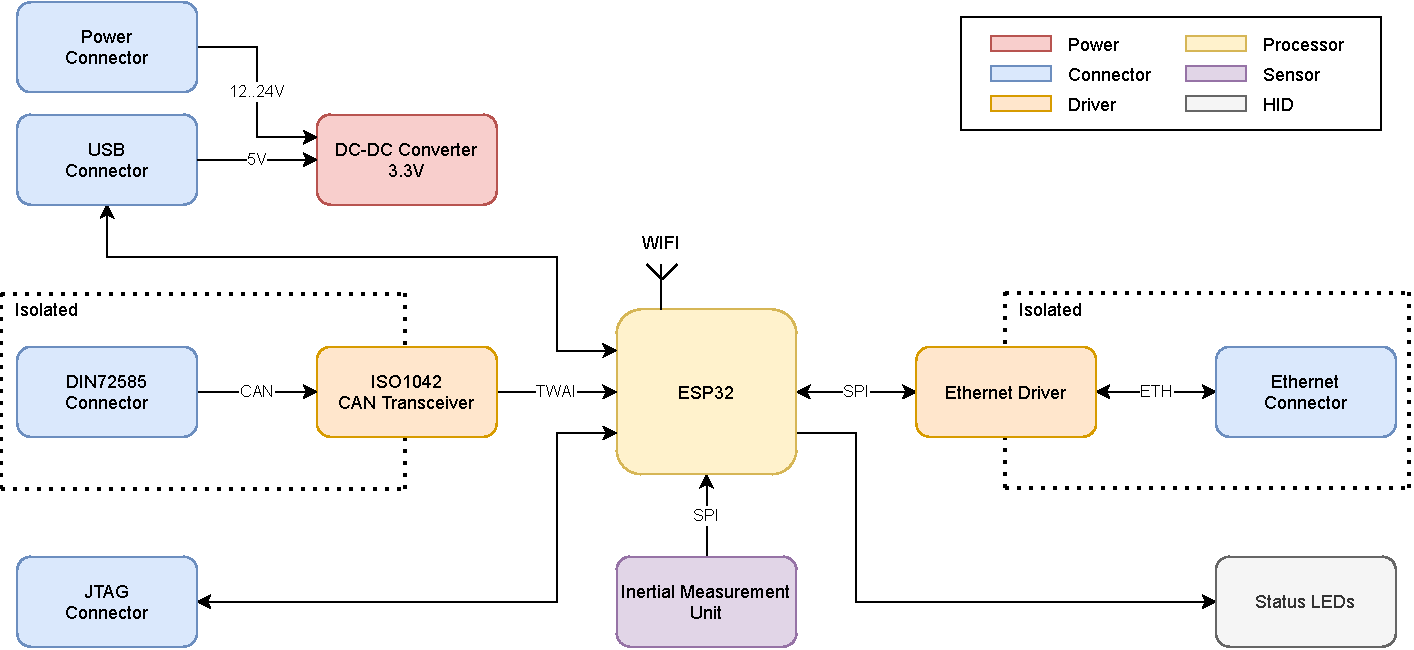
\includegraphics[height=7cm]{images/fleet_monitor_hardware}
	\caption{Hardware Block Diagram}
	%\vspace{-2ex}
	\label{fig:hardware_block_diagram}
\end{figure}

\newpage
\subsection{Protocol and Interface Standards}
The following protocol standards will be supported in this project:
\begin{itemize}
		\item \acrshort{wlan}-Interface: Wi-Fi 802,11b/g/n
		\item \acrshort{lan}-Interface: 10Base-T / 100Base-TX
		\item \acrshort{usb}-Interface: \acrshort{usb} 2.0 (Device)
		\item \acrshort{can}-Interface: \acrshort{sae} J1939
		\item \acrshort{fms}-Protocol: Version 04 (17.09.2021)
\end{itemize}

\label{sec:firmware}
\subsection{Firmware}
The embedded firmware will run on the \gls{esp32} and will be written in C. The requirements for the firmware are as follows:
\begin{itemize}
    \item The firmware shall read \acrshort{fms}-packages and prepare them for transmission.
    \item The firmware shall transmit the packages to the router.
    \subitem A filter shall be implemented to select the packages to be sent out.
    \subitem A filter shall be implemented to select the maximum update rate of a package.
    \subitem A filter shall be implemented to send data only on change.
    \item The firmware shall display the current device status to the user.
    \item The firmware shall read the \acrshort{imu}-data.
    \item The firmware shall transmit the \acrshort{imu}-data.
    \item The firmware should read a configuration file from the router (e.g. the filter of what packages shall be sent).
\end{itemize}

\subsection{Network Router Communication Tool}
The network router communication tool is the sole device communicating with the hardware. The system has the following requirements:
\begin{itemize}
        \item The system shall handle communication between the embedded system and the host.
        \item The system shall store the streamed data and make it available for further processing.
        \item The system should host files for the device (e.g. configuration file).
\end{itemize}

\subsection{Configuration File Creator}
The configuration file creator helps the user to easily change and adapt the behavior of the \acrshort{fms}-packet transmission. For each \acrshort{fms} command-type, specific filters can be applied (referenced in \cref{sec:firmware}). The configuration file creator fulfills the following requirements:
\begin{itemize}
        \item The file creator shall have the function to load and store configuration files.
        \item The file creator shall provide axes to change the filter settings.
\end{itemize}


\subsection{Graphical Visualizer (optional)}
This Python-based tool allows visualization of data that has been gathered and transmitted by the device.
It should be implemented as a stand-alone application which primarily can be used offline.
The graphical interface helps the user to easily understand the presented data.
The requirements for this tool are as follows:
\begin{itemize}
        \item The graphic visualizer shall open files containing \acrshort{fms} data packets.
        \item The graphic visualizer shall visualize user selected command-types.
\end{itemize}
